\chapter{放大电路的构建}
\textit{(本章的内容仅做了解)}

通过对BJT原理的分析,可以知道当BJT工作在放大区时,基极上一个很小的电流就可以引起集电极上一个较大电流的变化。本章将通过一个例子来说明如何利用这个特性来构造一个合理的放大电路。

\section{基本共射放大电路的构成}
想要利用BJT的放大特性来放大一个小信号,最简单的想法就是直接在BJT将信号源直接接在射极的两端,如图\ref{1}所示。但是实际中,$v_\mathrm{i}$的量级一般都是毫伏甚至更小,这样直接加在两端会导致发射结无法正偏。此时BJT没有工作在放大区,无法放大。

\begin{figure}[htb]
    \centering
    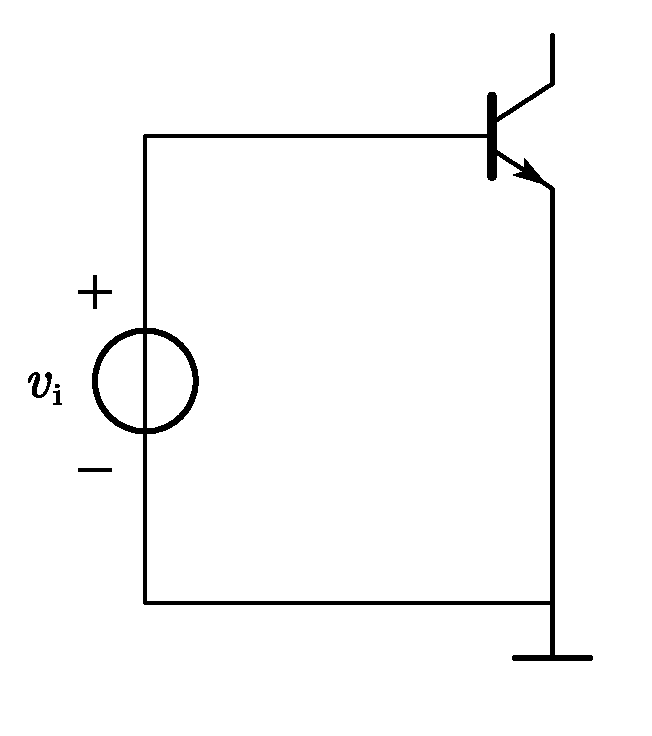
\includegraphics[width=0.35\linewidth]{pic/appendixApic/1.pdf}
    \caption{没有构建合理静态工作点的电路\label{1}}
\end{figure}

为了使BJT工作在放大区,需要在基极b和发射极e之间、集电极c和发射极e之间分别加上适当的直流电源$V_\mathrm{BB}$和$V_\mathrm{CC}$,使得发射结正偏、集电结反偏,如图\ref{2}所示。同时需要加入一个限流电阻$R_\mathrm{b}$避免be之间电压过大。

\begin{figure}[htb]
    \centering
        \subcaptionbox{静态工作点合理的电路\label{2}}
        {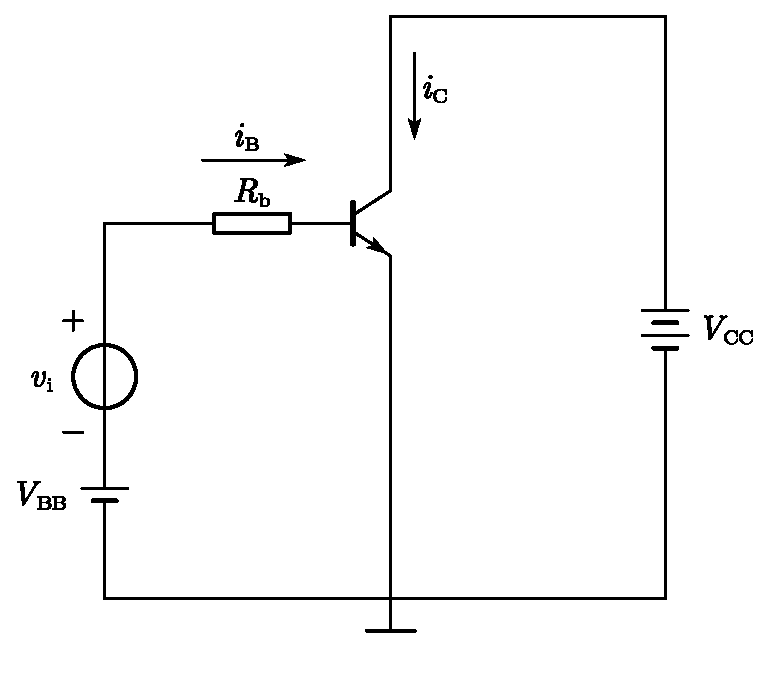
\includegraphics[width=0.35\linewidth]{pic/appendixApic/2.pdf}}\qquad
        \subcaptionbox{基本共射放大电路\label{3}}
        {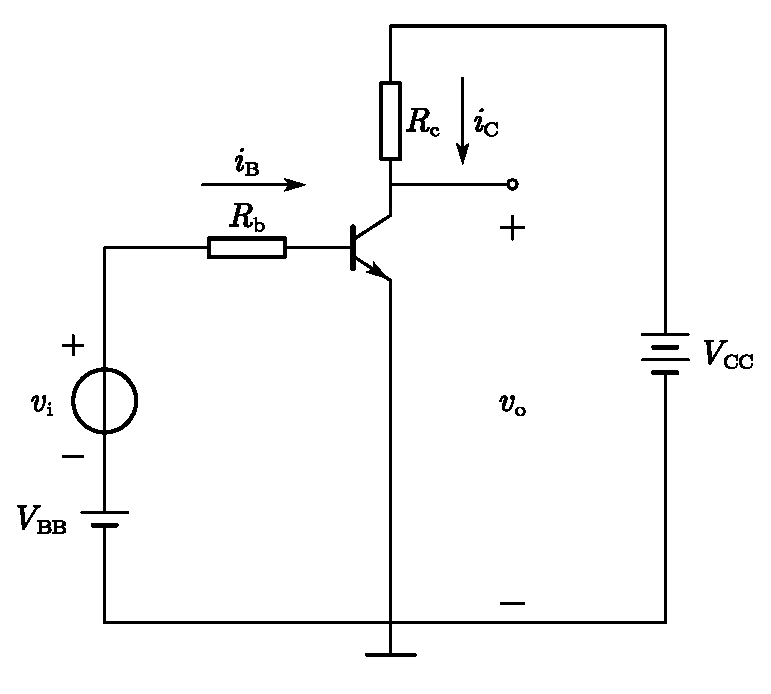
\includegraphics[width=0.35\linewidth]{pic/appendixApic/3.pdf}}
        \caption{基本共射放大电路的构成\label{静态工作点合理的电路}}
\end{figure}

通过构建合理的静态工作点,现在输入回路中$v_\mathrm{i}$引起$i_\mathrm{B}$的变化,会导致$i_\mathrm{C}$发生相应的变化。目前已经满足放大的所有要求了,但仍然存在一个问题——如何将$i_\mathrm{C}$的变化输出?最简单的思路是直接将负载接在$V_\mathrm{CC}$和BJT之间,但在实际操作中较为麻烦。另一种办法是在输出回路加上一个电阻$R_\mathrm{c}$,如图\ref{3}所示,将$i_\mathrm{C}$的变化转换为电压的变化,然后在集电极c和地之间输出。

\section{基本共射放大电路的改进}
通过以上的构造,就得到了基本共射放大电路,即第二章2.2.4小节中的图\ref{基本共射放大电路},现在希望优化其中的一些小细节。

电路存在的第一个问题是,电路中有两个电源$V_\mathrm{BB}$和$V_\mathrm{CC}$。实际上,只需要选择合适的$R_\mathrm{b}$和$R_\mathrm{c}$,就可以使得电源减少为一个,如图\ref{4}。稍作变化后可以得到图\ref{5}。
\begin{figure}[htb]
    \centering
        \subcaptionbox{变化前\label{4}}
        {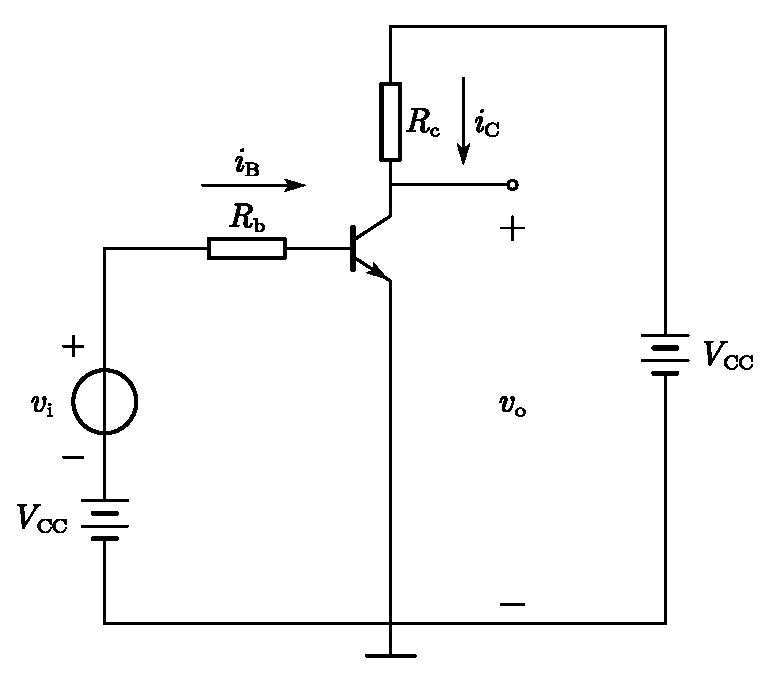
\includegraphics[width=0.35\linewidth]{pic/appendixApic/4.pdf}}\qquad
        \subcaptionbox{变化后\label{5}}
        {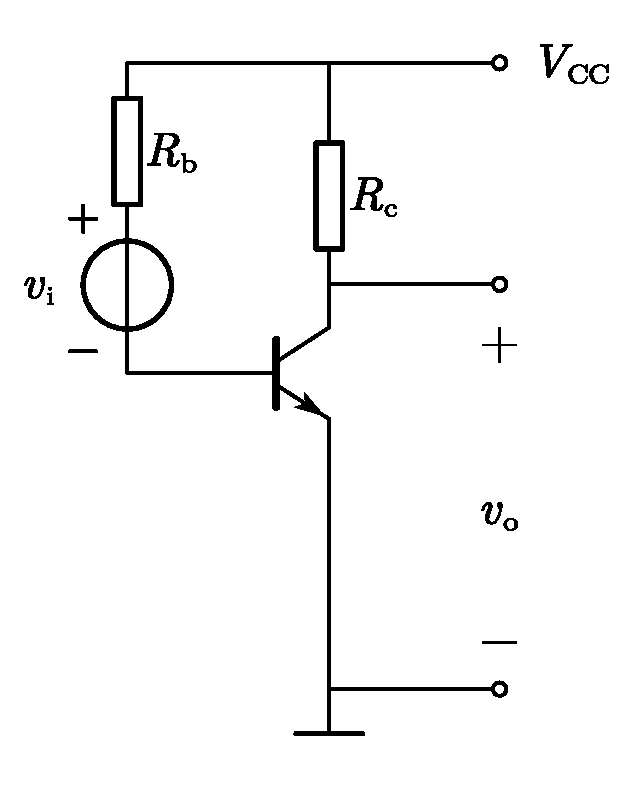
\includegraphics[width=0.25\linewidth]{pic/appendixApic/5.pdf}}
        \caption{减少电源数量后的放大电路\label{减少电源数量后的放大电路}}
\end{figure}

但是在变化后,电路出现了新的问题——此时的信号源变成了“浮地”状态,这样会对信号的传输造成一定不良的影响。如果想要信号源接到地上,最简单的思路就是将信号源直接接在基极b和发射极e之间。但是,这样又会造成BJT无法工作在放大状态,类似于图\ref{1}。

因此,需要引入$R_\mathrm{b1}$,使得电路有合适的静态工作点(这一点通过将$v_\mathrm{i}$置零就可以看出),如图\ref{6}所示。这种电路称为\textbf{直接耦合}的放大电路。

\begin{figure}[htb]
    \centering
    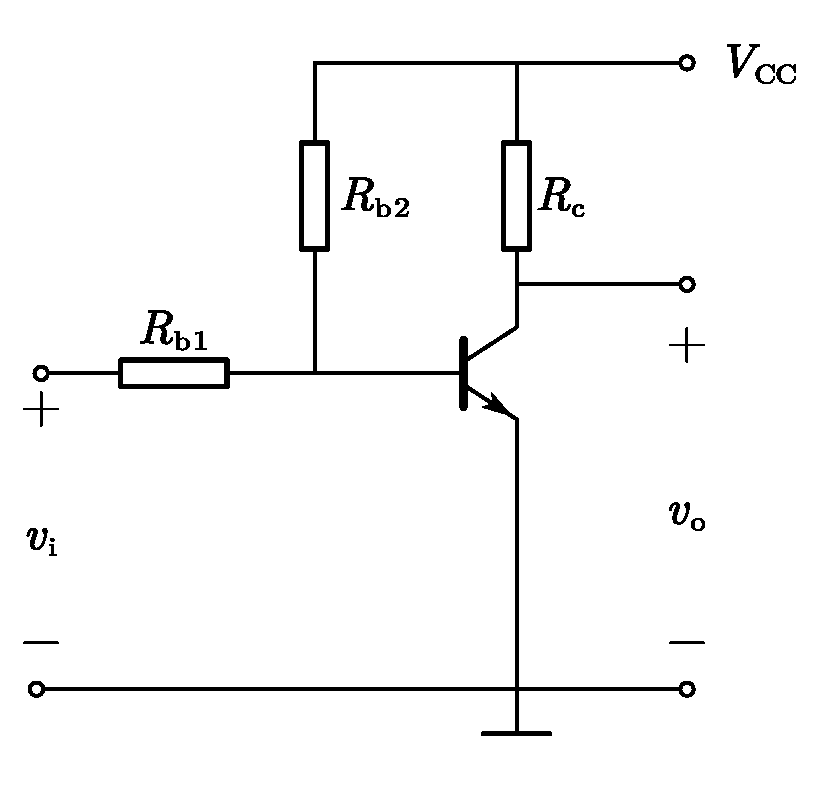
\includegraphics[width=0.35\linewidth]{pic/appendixApic/6.pdf}
    \caption{直接耦合的放大电路\label{6}}
\end{figure}

当引入的电阻$R_\mathrm{b1}$后,交流信号会在$R_\mathrm{b1}$和$R_\mathrm{b2}$上有一定分压,导致放大倍数降低,而在输出端,由于静态工作点的存在,输出的信号为直流信号和交流信号二者的叠加,常常需要去除。

因此,可以在输入输出端各引入一个电容,使得输入信号可以直接加在三极管的输入端,且输出的信号没有直流分量,如图\ref{7}所示。这种电路称为\textbf{阻容耦合}的放大电路。

\begin{figure}[htb]
    \centering
    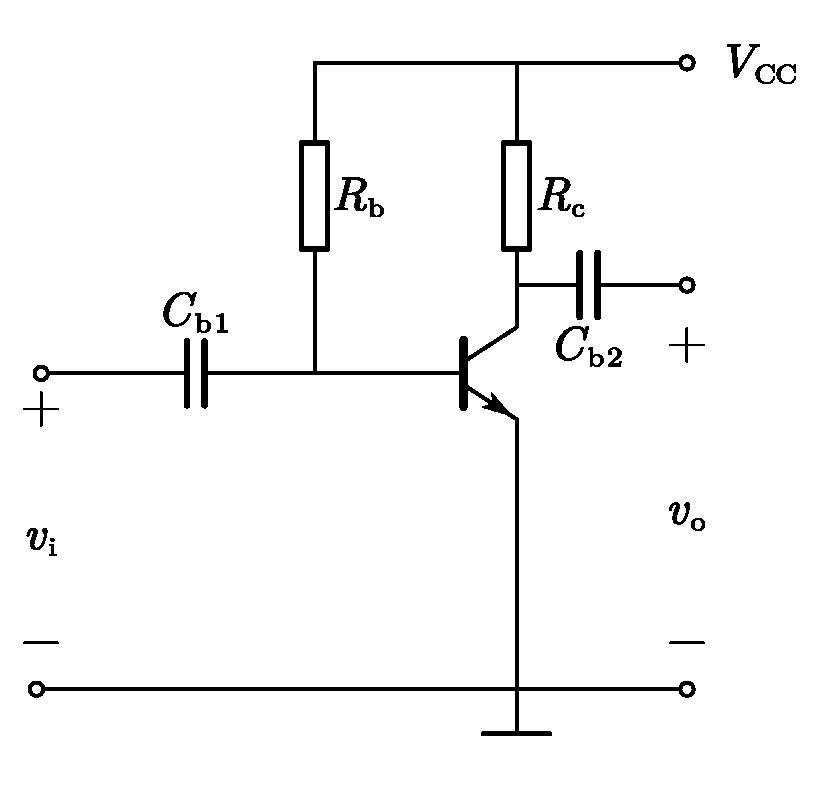
\includegraphics[width=0.35\linewidth]{pic/appendixApic/7.pdf}
    \caption{阻容耦合的放大电路\label{7}}
\end{figure}

\section{静态工作点的稳定}
静态工作点的稳定对于电路的放大至关重要,而温度往往是影响静态工作点的一个主要因素,温度的变化会导致静态工作点的漂移。

由BJT在不同温度下的工作特性曲线可以知道,温度上升,将会导致$i_\mathrm{C}$上升。如果能引入某个参数使得,在温度升高时使得$i_\mathrm{C}$下降,就能达到稳定静态工作点的目标。由于$i_\mathrm{C}$受到$v_{\mathrm{BE}}$控制,因此只需要让温度上升时$v_{\mathrm{BE}}$下降即可。

\begin{figure}[htb]
    \centering
        \subcaptionbox{引入负反馈后的电路\label{8}}
        {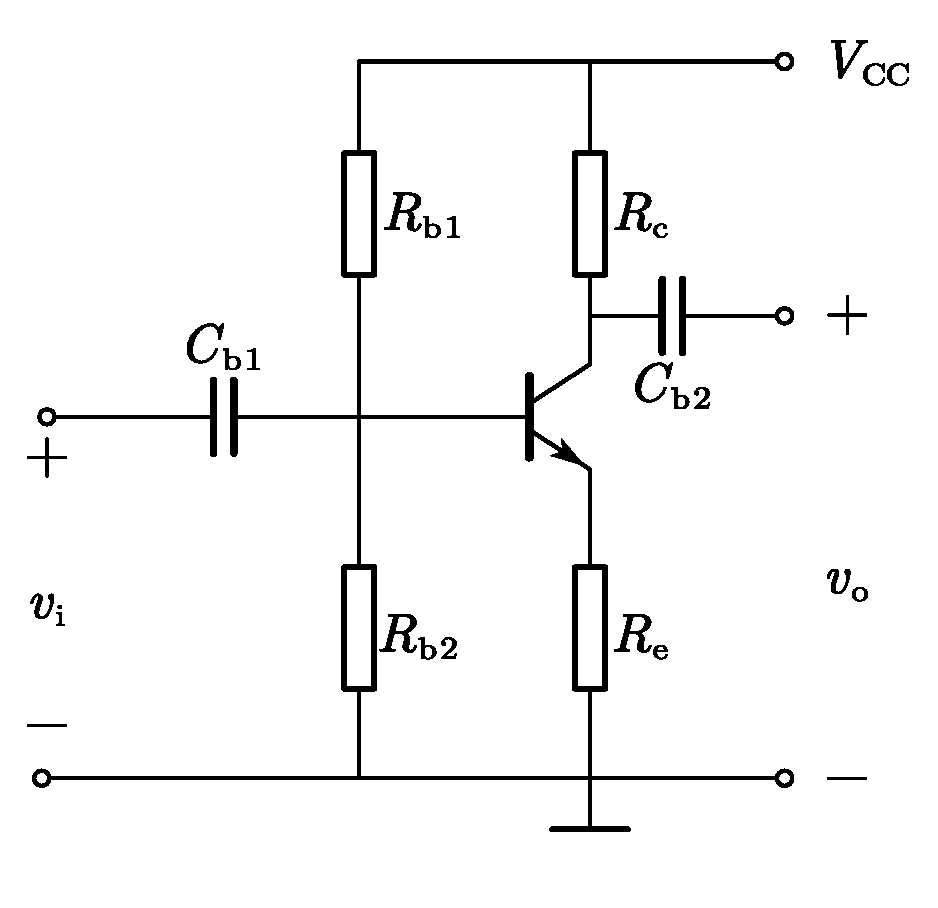
\includegraphics[width=0.35\linewidth]{pic/appendixApic/8.pdf}}\qquad
        \subcaptionbox{引入旁路电容后的电路\label{9}}
        {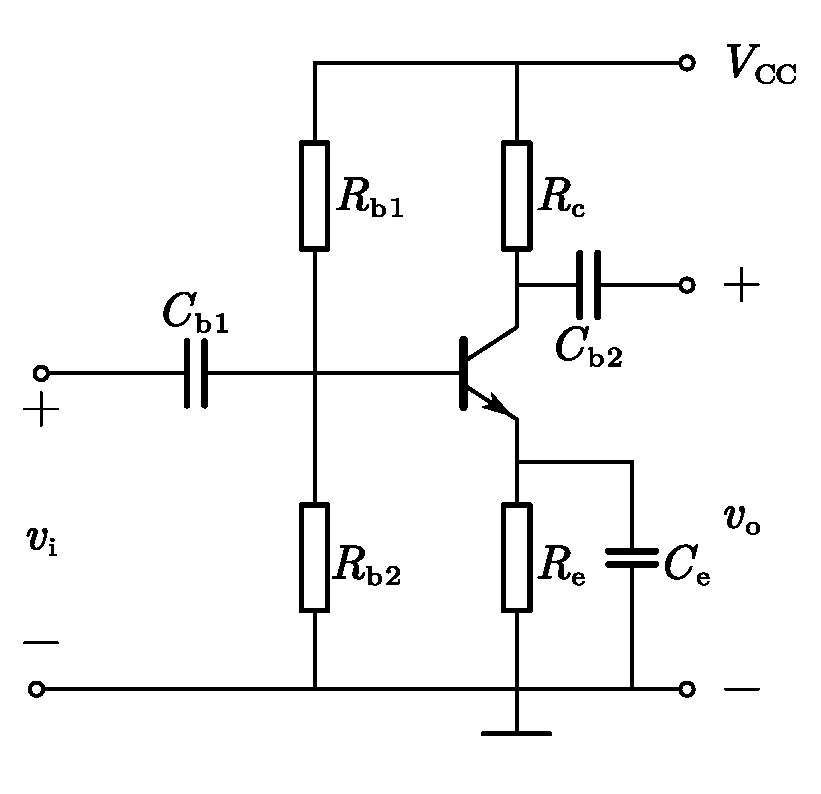
\includegraphics[width=0.35\linewidth]{pic/appendixApic/9.pdf}}
        \caption{静态工作点稳定的放大电路\label{静态工作点稳定的放大电路}}
\end{figure}

由图\ref{7}可以看出,静态情形下的射极电位已经是一个固定的值,无法随着$i_\mathrm{C}$的上升而改变。若此时在射极和接地点之间引入电阻$R_{\mathrm{e}}$,当$i_\mathrm{C}$上升时,射极电位$v_\mathrm{E}$随之上升,且变化量远大于基极电位$v_\mathrm{B}$变化。这样的一个负反馈机制就使得电路有一定的稳定性。

此外,为了使基极电位$v_\mathrm{B}$更稳定,可以在基极和接地点之间再引入一个电阻$R_{\mathrm{b2}}$,使得流经$R_{\mathrm{b2}}$的电流$i_{\mathrm{b2}}\gg i_{\mathrm{B}}$,则$v_\mathrm{B}$近似为两个电阻的分压,这样我们就得到了图\ref{8}。

由\ref{公式-共射放大电路增益}式,该电路的电压放大倍数为

\begin{equation}
    A_v=\frac{v_\mathrm{o}}{v_\mathrm{i}}=-\frac{\beta (R_\mathrm{c}\parallel R_\mathrm{L})}{r_\mathrm{be}+(1+\beta)R_\mathrm{e}}
\end{equation}

可以看出,$R_\mathrm{e}$导致电压的放大倍数降低了。为了使$R_\mathrm{e}$不出现在$A_v$的表达式中,可以在$R_\mathrm{e}$旁边并联一个\textbf{旁路电容}$C_\mathrm{e}$,此时在交流通路中$R_\mathrm{e}$就被短路了,如图\ref{9}所示。

这样,通过一步一步地分析问题、解决问题,就得到了一个性质较好的放大电路。